\documentclass[11pt]{article}
\usepackage[margin=1cm]{geometry}
\usepackage[portuguese]{babel}
\usepackage[utf8]{inputenc}
\usepackage{hyperref}
\usepackage{indentfirst}
\usepackage{subfig}
\usepackage{listings}
\usepackage{color}
\usepackage[export]{adjustbox}

\definecolor{dkgreen}{rgb}{0,0.6,0}
\definecolor{gray}{rgb}{0.5,0.5,0.5}
\definecolor{mauve}{rgb}{0.58,0,0.82}
\definecolor{codegreen}{rgb}{0,0.6,0}
\definecolor{codepurple}{rgb}{0.58,0,0.82}

\lstdefinestyle{mystyle}{
  commentstyle=\color{codegreen},
  % keywordstyle=\color{magenta},
  % stringstyle=\color{codepurple},
  basicstyle=\ttfamily\footnotesize,
  breakatwhitespace=false,
  breaklines=true,
  captionpos=b,
  keepspaces=true,
  numbers=left,
  numbersep=5pt,
  showspaces=false,
  showstringspaces=false,
  showtabs=false,
  tabsize=2
}
\lstset{style=mystyle}

\urlstyle{same}
\pagenumbering{gobble}
%\usepackage{multicol}
\hypersetup{
  colorlinks=true,
  linkcolor=black,
  filecolor=magenta,      
  urlcolor=blue,
  citecolor=black,
}
\usepackage[backend=bibtex]{biblatex}
\usepackage{graphicx}
\usepackage{tikz}
\pagestyle{plain}

\newcommand{\gaspar}{Diogo Gaspar, 99207}

\begin{document}
\begin{center}
{\huge{Exercício 9 - Projeto Computacional PE 2022}} \\
\vspace{1.5mm}
{\large{\gaspar}} \\
\end{center}

Consideremos como premissas que foram fixadas uma semente em 139, um conjunto de
tamanhos de amostras \{100, 200, ..., 5000\}.
O objetivo deste exercício passa por gerar 650 amostras com distribuição exponencial
de valor esperado $\frac{1}{\lambda} = \frac{1}{1.32}$ para cada tamanho supra-mencionado.
De seguida, construir para cada uma das amostras geradas um intervalo de confiança
aproximado para $\lambda$ (com intervalo de confiança $1 - \alpha = 0.93$), e para cada
tamanho de amostra calcular a média da amplitude de todos os intervalos de confiança
obtidos.

\vspace{0.5mm}
Para tal, recorreu-se ao seguinte trecho de código \texttt{R} (utilizando as bibliotecas \texttt{ggplot2, lattice, plyr} e \texttt{Rmisc}):

\begin{lstlisting}[language=R]
  set.seed(139)
  m <- 650
  lambda <- 1.32
  theoric_confidence_interval <- 0.93
  dimensions <- seq(100, 5000, 100)
  
  calculate_mean_widths <- function(n) {
    widths <- c()
    for (i in 1:m) {
      exp <- rexp(n, rate=lambda)
      confidence_interval <- CI(exp, ci=theoric_confidence_interval)
      widths <- c(widths, c(abs(confidence_interval[["upper"]] - confidence_interval[["lower"]])))
    }
    return (mean(widths))
  }
  
  mean_widths <- c()
  for (n in dimensions) {
    mean_widths <- c(mean_widths, calculate_mean_widths(n))
  }

  ggplot(data.frame(dimensions, mean_widths), aes(x=dimensions, y=mean_widths)) +
    geom_line(color="blue") +
    geom_point(color="blue") +
    theme_bw() +
    theme(axis.text.x = element_text(angle = 45, hjust = 1)) +
    xlab("Dimensão da amostra") + ylab("Amplitude média para 650 amostras") +
    ggtitle("Amplitude média dos intervalos de confiança da distribuição exponencial") +
    scale_x_continuous(breaks = round(seq(0, 5000, 500)))
\end{lstlisting}

\begin{tikzpicture}[remember picture, overlay]
  \node [shift = {(0cm, 4cm)}] at (current page.south)
    { 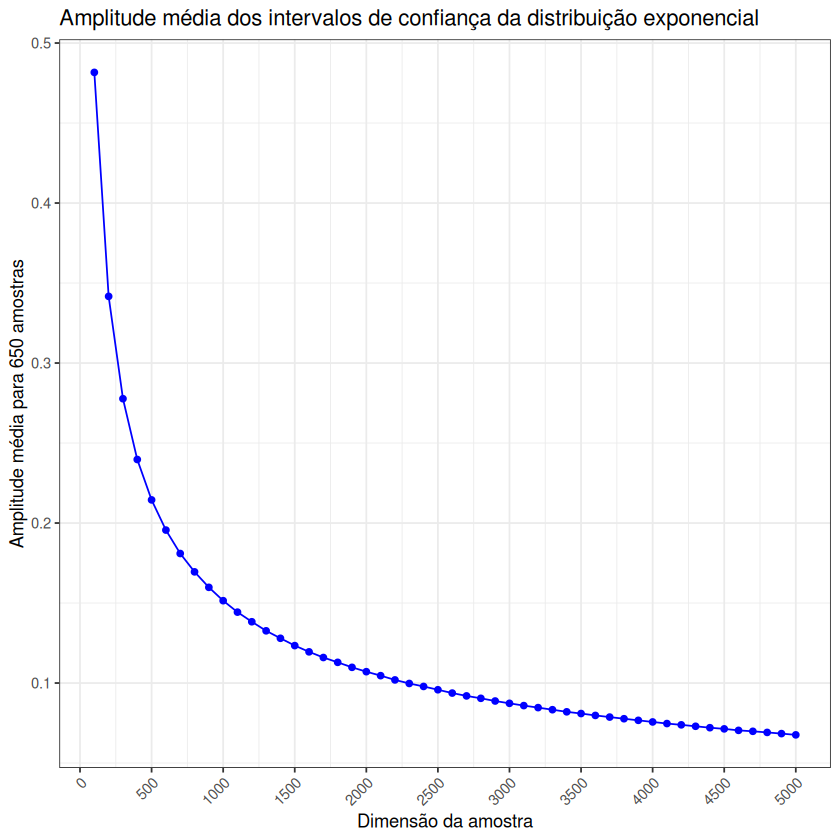
\includegraphics[scale = 0.45]{../imgs/exercise-9.png} };
\end{tikzpicture}

Note-se que à medida que o tamanho da amostra aumenta, a amplitude média entre intervalos
de confiança torna-se rapidamente mais pequena à medida que nos aproximamos de 5000.
Podemos, portanto, retirar deste gráfico que quanto maior o tamanho da população, mais
podemos \textbf{confiar} nos resultados obtidos, visto que vemos a amplitude média
dos intervalos de confiança a ser reduzida.

\end{document}